%%%%%%%%%%%%%%%%%%%%%%%%%%%%%%%%%%%%%%%%%
% Beamer Presentation
% LaTeX Template
% Version 1.0 (10/11/12)
%
% This template has been downloaded from:
% http://www.LaTeXTemplates.com
%
% License:
% CC BY-NC-SA 3.0 (http://creativecommons.org/licenses/by-nc-sa/3.0/)
%
%%%%%%%%%%%%%%%%%%%%%%%%%%%%%%%%%%%%%%%%%

%----------------------------------------------------------------------------------------
%	PACKAGES AND THEMES
%----------------------------------------------------------------------------------------


\documentclass[brazil]{beamer}

\usepackage{graphicx} % Allows including images
\usepackage{booktabs} % Allows the use of \toprule, \midrule and \bottomrule in tables
\usepackage[utf8]{inputenc}
\usepackage[T1]{fontenc}
\usepackage[brazil]{babel}
\usepackage{subfig}
\usepackage{xcolor,graphicx,tikz,url}
\usepackage{pbox}
\usepackage{adjustbox}
\usepackage{listings, lstautogobble}

\renewcommand{\lstlistingname}{Código}

\lstset{
	frame=single,
	breaklines=true,
	postbreak=\raisebox{0ex}[0ex][0ex]{\ensuremath{\color{red}\hookrightarrow\space}},
	autogobble=true
}

\mode<presentation> {

% The Beamer class comes with a number of default slide themes
% which change the colors and layouts of slides. Below this is a list
% of all the themes, uncomment each in turn to see what they look like.

\usetheme{default}
%\usetheme{AnnArbor}
%\usetheme{Antibes}
%\usetheme{Bergen}
%\usetheme{Berkeley}
%\usetheme{Berlin}
%\usetheme{Boadilla}
%\usetheme{CambridgeUS}
%\usetheme{Copenhagen}
%\usetheme{Darmstadt}
%\usetheme{bjeldbak}
%\usetheme{Dresden}
%\usetheme{Frankfurt}
%\usetheme{Goettingen}
%\usetheme{Hannover}
%\usetheme{Ilmenau}
%\usetheme{JuanLesPins}
%\usetheme{Luebeck}
%\usetheme{Madrid}
%\usetheme{Malmoe}
%\usetheme{Marburg}
%\usetheme{Montpellier}
%\usetheme{PaloAlto}
%\usetheme{Pittsburgh}
%\usetheme{Rochester}
%\usetheme{Singapore}
%\usetheme{Szeged}
%\usetheme{Warsaw}

% As well as themes, the Beamer class has a number of color themes
% for any slide theme. Uncomment each of these in turn to see how it
% changes the colors of your current slide theme.

%\usecolortheme{albatross}
%\usecolortheme{beaver}
%\usecolortheme{beetle}
%\usecolortheme{crane}
%\usecolortheme{dolphin}
%\usecolortheme{dove}
%\usecolortheme{fly}
%\usecolortheme{lily}
%\usecolortheme{orchid}
%\usecolortheme{rose}
%\usecolortheme{seagull}
%\usecolortheme{seahorse}
%\usecolortheme{whale}
%\usecolortheme{wolverine}

%\setbeamertemplate{footline} % To remove the footer line in all slides uncomment this line
%\setbeamertemplate{footline}[page number] % To replace the footer line in all slides with a simple slide count uncomment this line

%\setbeamertemplate{navigation symbols}{} % To remove the navigation symbols from the bottom of all slides uncomment this line
}


%----------------------------------------------------------------------------------------
%	TITLE PAGE
%----------------------------------------------------------------------------------------

\title[Bolsa Família e Cassandra]{Armazenamento de Dados Abertos com NoSQL: Um estudo de caso com Dados do Bolsa Família e NoSQL Cassandra} % The short title appears at the bottom of every slide, the full title is only on the title page

\author{Jorge Luiz Andrade} % Your name
\institute[UnB] % Your institution as it will appear on the bottom of every slide, may be shorthand to save space
{
Universidade de Brasília \\ % Your institution for the title page
\medskip
\textit{jorgeluizandrade@outlook.com} % Your email address
}
\date{\today} % Date, can be changed to a custom date

\begin{document}

\begin{frame}
\titlepage % Print the title page as the first slide
\end{frame}

% \begin{frame}
% \frametitle{Sumário} % Table of contents slide, comment this block out to remove it
% \tableofcontents % Throughout your presentation, if you choose to use \section{} and \subsection{} commands, these will automatically be printed on this slide as an overview of your presentation
% \end{frame}

%----------------------------------------------------------------------------------------
%	PRESENTATION SLIDES
%----------------------------------------------------------------------------------------

%------------------------------------------------
\section{Introdução} 
%------------------------------------------------
\begin{frame}

\frametitle{Introdução}
\end{frame}

\begin{frame}
\frametitle{Introdução}

\end{frame}

\begin{frame}
\frametitle{Introdução}
\vfill


\begin{block}{Problema}
	Banco de Dados Relacionais podem não apresentar um desempenho satisfatório ao operar grandes volumes de dados
\end{block}
\vfill

\onslide<2->{%
\begin{block}{Hipótese}
	O uso de múltiplas máquinas em um ambiente Cassandra distribuído pode oferecer um melhora do desempenho que justifique sua utilização na análise de dados abertos.	
\end{block}}
\vfill

\end{frame}

\begin{frame}
\frametitle{Introdução}

\begin{block}{Objetivos}
	Comparar o desempenho de um banco Cassandra para inserções e consultas em diferentes tamanhos de \emph{cluster} e de volumes de dados;
	
	\begin{itemize}
		\item Desenvolver uma aplicação para inserção e busca dos dados do Bolsa Família;
		\item Realizar testes de inserção e busca com diferentes configurações;
		\item Comparar o desempenho do Cassandra nas diferentes situações;
	\end{itemize}
\end{block}
\end{frame}

%------------------------------------------------
\section{Fundamentação Teórica}
%------------------------------------------------

% \subsection{Dados Abertos}

% \begin{frame}
% \end{frame}

%------------------------------------------------

\subsection{Bancos de Dados}

\begin{frame}
\frametitle{Bancos Relacionais}
	\begin{itemize}
		\item Proposto em 1970 por Edgar Codd;
		\item Conjunto de relações entre tuplas;
	\end{itemize}
\end{frame}

\begin{frame}
\frametitle{Propriedades ACID}
	\begin{itemize}
		\item Atomicidade;
		\item Consistência;
		\item Isolamento;
		\item Durabilidade;
	\end{itemize}
	Garantem a validade do esquema, mas sacrificam desempenho e disponibilidade.
\end{frame}


\begin{frame}
\frametitle{Normalização}
	\begin{itemize}
		\item \textbf{1FN}: Cada coluna deve guardar apenas uma informação(valores atômicos);
		\item \textbf{2FN}: Atributos não-chave devem depender integralmente da chave primária da tabela;
		\item \textbf{3FN}: Atributos não-chave não podem ser determinados por outros atributos não-chave; 
	\end{itemize}
\end{frame}

\subsection{NoSQL}
Modelos relacionais possuem restrições, como as propriedades ACID e Normalização, gerando problemas de escalabilidade e rigidez de esquema.
\begin{frame}
\frametitle{NoSQL}
	\begin{itemize}
		\item Termo utilizado pela primeira vez em 1998(Strozzi NoSQL)
		\item Google Bigtable(2006) e Amazon's Dynamo(2007)
	\end{itemize}
\end{frame}


\begin{frame}
	\frametitle{Teorema CAP}
	\begin{itemize}
		\item Proposto em 2000 por Eric Brewer, define limitações em sistemas distribuídos;
		\item Revisado em 2012;
		\item Consistência;
		\item Disponibilidade;
		\item Tolerância a partições
	\end{itemize}
\end{frame}

\subsection{Modelos NoSQL}
\begin{frame}
	\frametitle{Chave-Valor}
		Consiste em uma tabela \emph{hash}, com consultas a um valor a partir de uma chave.
		\begin{itemize}
			\item Berkeley DB;
			\item Amazon DynamoDB;
		\end{itemize}
\end{frame}

\begin{frame}
	\frametitle{Documentos}
		Acesso à um documento de esquema flexível a partir de uma chave.
		\begin{itemize}
			\item CouchDB;
			\item MongoDB;
		\end{itemize}
\end{frame}

\begin{frame}
	\frametitle{Grafos}
		Dados altamente conectados, com consultas baseadas em relacionamentos.
		\begin{itemize}
			\item Neo4j
			\item OrientDB
		\end{itemize}
\end{frame}

\begin{frame}
	\frametitle{Colunas}
		Dados armazenados em famílias de colunas. Possui esquema flexível, permitindo a modificação de colunas a qualquer momento.
		\begin{itemize}
			\item HBase
			\item \textbf{Cassandra}
		\end{itemize}
\end{frame}

%------------------------------------------------
\section{Cassandra}


%------------------------------------------------
\section{Metodologia}
\begin{frame}
	\frametitle{Programa Bolsa Família}
	Programa de transferência de renda criado em 2003. 
	
	Em 2016, atendia 13,9 milhões de famílias, que recebiam uma média de R\$ cada, totalizando R\$27,4 bilhões.
	
	\begin{itemize}
		\item Dados disponibilizados no Portal da Transparência;
		\item Arquivos mensais em formato .csv;
	\end{itemize}
\end{frame}

\begin{frame}
	\frametitle{Dados Utilizados}
	Foram utilizados um total de trinta arquivos, referentes aos meses de Julho de 2014 a Dezembro de 2016. Os arquivos totalizam 16Gib de tamanho e cerca de 14 mil registros.
	
	\begin{table}
		\centering
		\adjustbox{max height=\dimexpr\textheight-7cm\relax,
			max width=\textwidth}{
		\begin{tabular}{|l|c|c|}
			\hline
			\textbf{Campo}         & \textbf{Tipo} & \textbf{Utilizado} \\ \hline
			UF                     & Text          & Sim                \\ \hline
			Código SIAFI Município & Int           & Sim                \\ \hline
			Nome Município         & Text          & Sim                \\ \hline
			Código Função          & -             & Não                \\ \hline
			Código Subfunção       & -             & Não                \\ \hline
			Código Programa        & -             & Não                \\ \hline
			Código Ação            & -             & Não                \\ \hline
			NIS Favorecido         & Bigint        & Sim                \\ \hline
			Nome Favorecido        & Text          & Sim                \\ \hline
			Fonte-Finalidade       & Text          & Sim                \\ \hline
			Valor Parcela          & Double        & Sim                \\ \hline
			Mês Competência        & Timestamp     & Sim                \\ \hline
		\end{tabular}
		}
	\end{table}
	
\end{frame}

\begin{frame}[fragile]
	\frametitle{Modelo de Dados}
	\begin{itemize}
		\item Fator de replicação de 1 (sem tolerância a falhas);
		\item \emph{SimpleStrategy} (\emph{datacenter} único);
		\item Criação do ambiente com uso de CQL;
	\end{itemize}

	\begin{tabular}{c}
	\begin{lstlisting}[caption={Código CQL para criação do keyspace},label={lst:cql_create_table},language=SQL]
	CREATE KEYSPACE bolsa_familia WITH replication = {'class': 'SimpleStrategy', 'replication_factor': 1};
	\end{lstlisting}
	\end{tabular}

	\begin{tabular}{c}
	\begin{lstlisting}[caption={Código CQL para criação da tabela},label={lst:cql_create_table},language=SQL]
		CREATE TABLE bolsa_familia.dados (uf TEXT, periodo TIMESTAMP, valor DOUBLE, nis_favorecido BIGINT, cod_municipio INT, fonte TEXT, nome_favorecido TEXT, nome_municipio TEXT, PRIMARY KEY(nis_favorecido, periodo, valor));
	\end{lstlisting}
	\end{tabular}

\end{frame}

\begin{frame}[fragile]
		\frametitle{Arquitetura do Ambiente}
		\begin{itemize}
			\item \emph{Cluster} composto por seis máquinas Intel i5-4570 3.20GHz, 16GB de RAM, disco rígido de 500GB, com sistema operacional Ubuntu;
			\item Cliente Cassandra versão 3.0.4;
			\item Configuração do arquivo \emph{cassandra.yaml};
		\end{itemize}
	
		\begin{tabular}{c}
			\begin{lstlisting}[caption={Configuração cassandra.yaml},language=python]
			cluster_name: 'BolsaFamilia Cluster C2M FR1'
			
			num_tokens: 256
			
			partitioner: org.apache.cassandra.dht.Murmur3Partitioner
			
			seed_provider:
			- class_name: org.apache.cassandra.locator.SimpleSeedProvider
			parameters:
			- seeds: "164.41.40.35"
			
			endpoint_snitch: SimpleSnitch
			\end{lstlisting}
		\end{tabular}
	
		Configurações do Linux:
		\begin{itemize}
			\item Remoção do limite de memória;
			\item Aumento do limite do número de arquivos abertos;
			\item Desativação do \emph{swap};
		\end{itemize}
\end{frame}

\begin{frame}
	\frametitle{Desenvolvimento da Aplicação}
	
	Foi desenvolvida uma aplicação em Java responsável pela leitura dos arquivos de entrada, inserção no banco e busca de dados:
	\begin{itemize}
		\item \emph{Driver} \emph{Datastax};
		\item Tratamento e filtragem dos campos;
		\item Interações com o banco por meio de CQL;
	\end{itemize}

	 \begin{figure}
		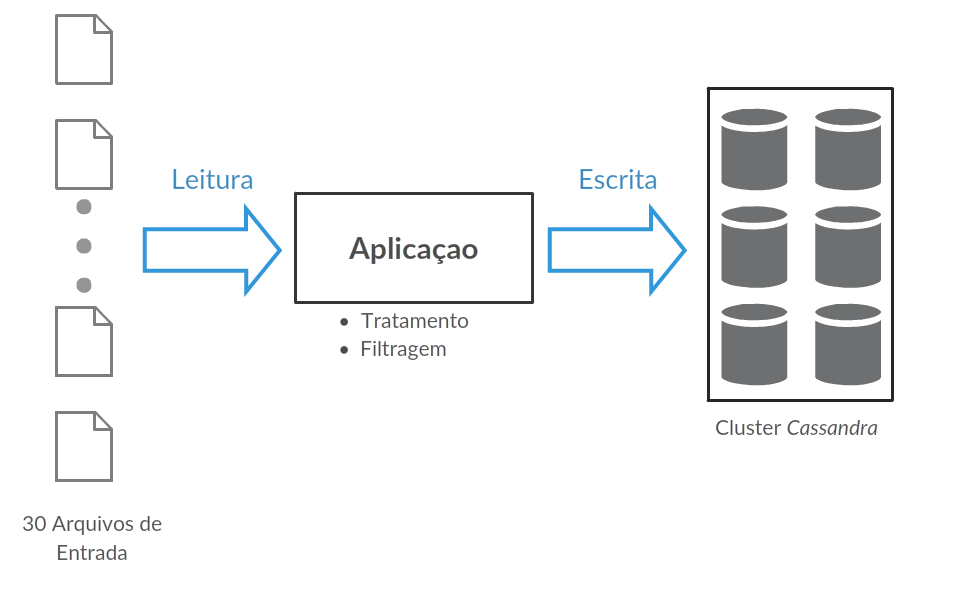
\includegraphics[width=0.7\linewidth]{figuras/aplicacao.png}
		\caption{Esquema da aplicação desenvolvida}
	\end{figure}
\end{frame}

%------------------------------------------------
\section{Resultados}

\subsection{Carga de Dados}
\begin{frame}
	\frametitle{Carga dos Dados}
	A aplicação desenvolvida realiza a filtragem dos campos e tratamento dos valores:
	\begin{itemize}
		\item Remoção do separador de milhares(,) em Valor Parcela;
		\item Alteração do padrão de data de MM/AAAA para DD/MM/AAAA;		
	\end{itemize}

	Foi realizada a carga com dois volumes de dados, correspondentes a dezoito e trinta meses do programa Bolsa Família.
	\begin{table}
		\centering
		\caption{Volume de dados}
		\adjustbox{max height=\dimexpr\textheight-7cm\relax,
			max width=\textwidth}{
			\begin{tabular}{ll}
			\textbf{Carga} & \textbf{Tamanho} \\ \hline
			18 meses       &  8,79 GB         \\ \hline
			30 meses       &  14,69 GB        \\ \hline
			\end{tabular}
		}
	\end{table}	
\end{frame}

\begin{frame}[fragile]
	\frametitle{Carga dos Dados}
	Inserção realizada com uso do \emph{driver} da \emph{Datastax}, por meio de query CQL, tendo seus parâmetros substituídos.
	
	\begin{tabular}{c}
		\begin{lstlisting}[caption={Código CQL para inserção},language=SQL]
			INSERT INTO bolsa_familia.dados (uf, cod_municipio, nome_municipio, nis_favorecido, nome_favorecido, fonte, valor, periodo) VALUES (?, ?, ?, ?, ?, ?, ?, ?)
		\end{lstlisting}
	\end{tabular}
\end{frame}

\begin{frame}
	\frametitle{Tempos de Inserção}
	
		\begin{table}
		\centering
		\caption{Tempos de Inserção}
		\adjustbox{max height=\dimexpr\textheight-7cm\relax,
			max width=\textwidth}{
			\begin{tabular}{lllll}
			\textbf{Volume}		& \textbf{2 nós} & \textbf{4 nós} & \textbf{6 nós} \\ \hline
			\textbf{18 meses}   & 1h         	 & 55m       	  & 52m            \\ \hline
			\textbf{30 meses}   & 2h31m      	 & 2h19m          & 2h06m          \\ \hline
			\end{tabular}
		}
		\end{table}	
	
		\begin{table}
			\centering
			\caption{Comparativo}
			\adjustbox{max height=\dimexpr\textheight-7cm\relax,
				max width=0.8\textwidth}{
				\begin{tabular}{lllll}
				\textbf{Volume} 	& \textbf{2 para 4 máquinas} & \textbf{4 para 6 máquinas} & \textbf{Média}  &  \\ \hline
				\textbf{18 meses} 	& 8,70\%                     & 4,22\%                     & \textbf{6,46\%} &  \\ \hline
				\textbf{30 meses}	& 8,13\%                     & 8,94\%                     & \textbf{8,54\%} &  \\ \hline
				\end{tabular}
			}
		\end{table}	
	
\end{frame}

\begin{frame}
	\frametitle{Tempos de Inserção}
	
	\begin{figure}
		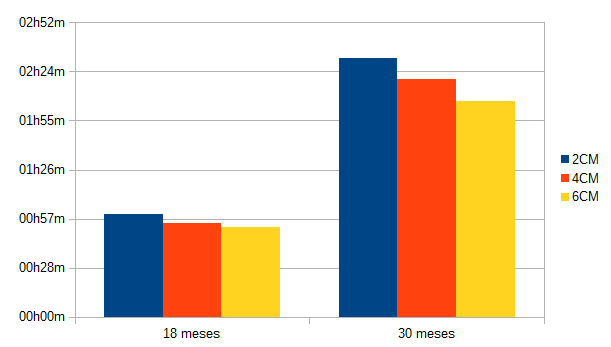
\includegraphics[width=0.7\linewidth]{figuras/graphinsert.png}
		\caption{Tempos de Inserção}
	\end{figure}
\end{frame}

\begin{frame}[fragile]
	\frametitle{Consultas}
	
	As consultas também foram realizadas por meio do \emph{driver} da \emph{Datastax}. Foram realizadas 30 consultas, buscando um registro específico por chave primária de forma aleatória.
	
	\begin{tabular}{c}
		\begin{lstlisting}[caption={Código CQL para consulta},language=SQL]
		SELECT * FROM dados WHERE nis_favorecido = 00020915229557 AND periodo = '2014-07-01' AND valor = 147.00 
		\end{lstlisting}
	\end{tabular}
\end{frame}

\begin{frame}
	\frametitle{Tempos de Consulta}
	
	\begin{table}
		\centering
		\caption{Tempos de Consulta}
		\adjustbox{max height=\dimexpr\textheight-7cm\relax,
			max width=\textwidth}{
			\begin{tabular}{lllll}
				\textbf{Volume}		& \textbf{2 nós} & \textbf{4 nós} & \textbf{6 nós} \\ \hline
				18 meses         & 10,26 s        & 1,95 s        & 1,73 s        \\ \hline
				30 meses         & 12,98 s        & 4,38 s        & 1,43 s         \\ \hline
			\end{tabular}
		}
	\end{table}	
	
	\begin{table}
		\centering
		\caption{Comparativo}
		\adjustbox{max height=\dimexpr\textheight-7cm\relax,
			max width=0.8\textwidth}{
			\begin{tabular}{lllll}
				\textbf{Volume} 	& \textbf{2 para 4 máquinas} & \textbf{4 para 6 máquinas}  & \textbf{Média}   &  \\ \hline
				\textbf{18 meses} 	& 81,00\%                    & 11,41\%                     & \textbf{46,20\%} &  \\ \hline
				\textbf{30 meses}	& 66,21\%                    & 67,48\%                     & \textbf{66,85\%} &  \\ \hline
			\end{tabular}
		}
	\end{table}	
\end{frame}

\begin{frame}
	\frametitle{Tempos de Consulta}
	
	\begin{figure}
		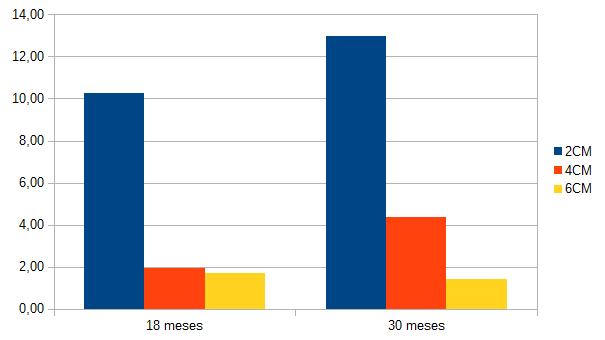
\includegraphics[width=0.7\linewidth]{figuras/graphselect.png}
		\caption{Tempos de Consulta}
	\end{figure}
\end{frame}

%------------------------------------------------
\section{Conclusão}
\begin{frame}
\frametitle{Resultados}
	Comparação do aumento do número de máquinas:
\begin{itemize}
	\item Melhora média de 7,5\% na inserção dos dados;
	\item Melhora média de 56,53\% na busca dos dados;
\end{itemize}
\end{frame}

\subsection{Trabalhos futuros}
\begin{frame}
\frametitle{Trabalhos futuros}
\begin{itemize}
	\item Isolamento da rede no ambiente utilizado;
	\item Comparação com outros bancos;
	\item Implementar diferentes modelagens no banco Cassandra;
\end{itemize}


\end{frame}
%------------------------------------------------

%------------------------------------------------
\subsection{Bibliografia}
\begin{frame}
\frametitle{Bibliografia}\footnotesize
  \nocite{}
  \bibliography{bibliografia}
  \bibliographystyle{plain}
\end{frame}


%----------------------------------------------------------------------------------------

\end{document} 
